% ============================================================
%  1-bit register - block symbol.
%  A D flip-flop with a load enable (LD): captures D on the clock
%  edge when LD=1, holds its value when LD=0.
%  Compile:  pdflatex symbol.tex
% ============================================================
\documentclass[border=14pt]{standalone}
\usepackage{tikz}
\usepackage{amsmath}
\begin{document}
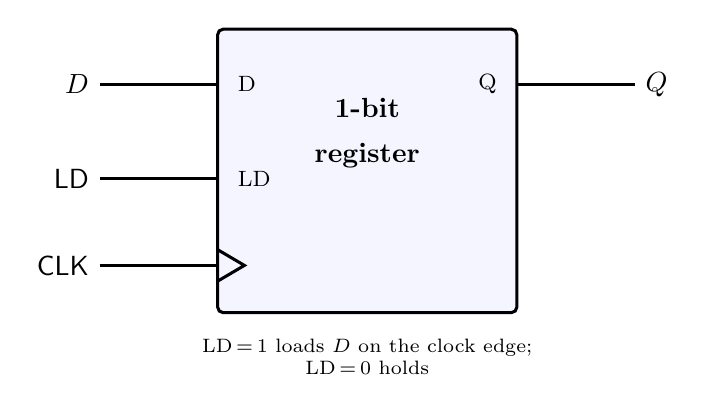
\begin{tikzpicture}[line width=1.1pt, font=\sffamily]
  \draw[rounded corners=2pt, fill=blue!4] (0,0) rectangle (3.8,3.6);
  \node[font=\bfseries] at (1.9,2.6) {1-bit};
  \node[font=\bfseries] at (1.9,2.0) {register};

  % inputs
  \draw (-1.5,2.9) node[left]{$D$}   -- (0,2.9);
  \draw (-1.5,1.7) node[left]{LD}    -- (0,1.7);
  \draw (-1.5,0.6) node[left]{CLK}   -- (0,0.6);
  \draw (0,0.4) -- (0.34,0.6) -- (0,0.8);          % edge-trigger triangle
  \node[anchor=west,font=\footnotesize] at (0.12,2.9) {D};
  \node[anchor=west,font=\footnotesize] at (0.12,1.7) {LD};

  % output
  \draw (3.8,2.9) -- (5.3,2.9) node[right]{$Q$};
  \node[anchor=east,font=\footnotesize] at (3.68,2.9) {Q};

  \node[font=\scriptsize,anchor=north,align=center] at (1.9,-0.2)
        {LD\,=\,1 loads $D$ on the clock edge;\\ LD\,=\,0 holds};
\end{tikzpicture}
\end{document}
